\documentclass[11pt,a4paper,twocolumn]{article}
\usepackage[utf8]{inputenc}
\usepackage{amsmath}
\usepackage{amssymb}
\usepackage{geometry}
\usepackage{cite}
\usepackage{microtype}
\usepackage{graphicx}
\usepackage{hyperref}
\usepackage{booktabs}

\geometry{margin=0.75in}

\title{\textbf{Early-Time Confinement Energy from Brane Rupture and the Hubble Tension: A Real-Data Test of Viability}}
\author{\textbf{Paul Jarvis} \\
\small Independent Researcher, UK \\
\small \texttt{mrpaulwjarvis@gmail.com} \\
\small ORCID: 0009-0009-8933-857X}
\date{\small August 17, 2026}

\begin{document}

\maketitle

\begin{abstract}
We test whether a transient early-time confinement-release energy component, motivated by higher-dimensional brane rupture dynamics, can resolve the Hubble tension against real cosmological data. Using a confinement-energy function $f(x) = x^\alpha(1-x)^\beta$ coupled to a tanh-triggered transition in scale factor, we perform a joint fit to DESI DR2 baryon acoustic oscillation measurements, Planck 2018 compressed CMB distance priors, the SH0ES local $H_0$ measurement, and the Planck 2018 constraint on the effective number of relativistic species $N_{\rm eff}$. At the fiducial profile shape ($\alpha = 4$, $\beta = 8$), the confinement mechanism removes essentially all of the tension: $\Delta\chi^2 = -16.0$ relative to $\Lambda$CDM, with a best-fit $H_0 = 73.10\ {\rm km\,s^{-1}\,Mpc^{-1}}$, matching SH0ES almost exactly, confirmed by a full MCMC posterior. This is a real, non-trivial phenomenological result. It requires, however, a peak confinement fraction $\rho_0 = 0.203$, roughly twice a Planck-safe bound of $0.1$ not traceable to any specific citation in the literature; the closest real literature analog, from early dark energy studies of Planck data alone, is the tighter bound $f_{\rm EDE} < 0.087$ at 95\% confidence. The resulting equation of state also violates the causal bound $w \leq 1$ severely, reaching $w_{\rm conf} \simeq 11$ at recombination and peaking near $77$. Extending the search to the full confinement profile family, letting $\alpha$, $\beta$, and the transition width $\Delta a$ vary jointly with the fit, does not rescue the mechanism: no point in this space is simultaneously causal and capable of resolving the tension. The best causally-respecting point found in the full family achieves only $H_0 = 70.6$, about one third of the way from $\Lambda$CDM to SH0ES, and requires an even larger confinement fraction, $\rho_0 = 0.95$. We conclude that the confinement-release profile is a genuine phenomenological fit to real cosmological data, but is excluded as a physically viable mechanism for resolving the Hubble tension across its full natural parameter space, not merely at one particular choice of shape parameters.
\end{abstract}

\begin{figure*}[t]
\centering
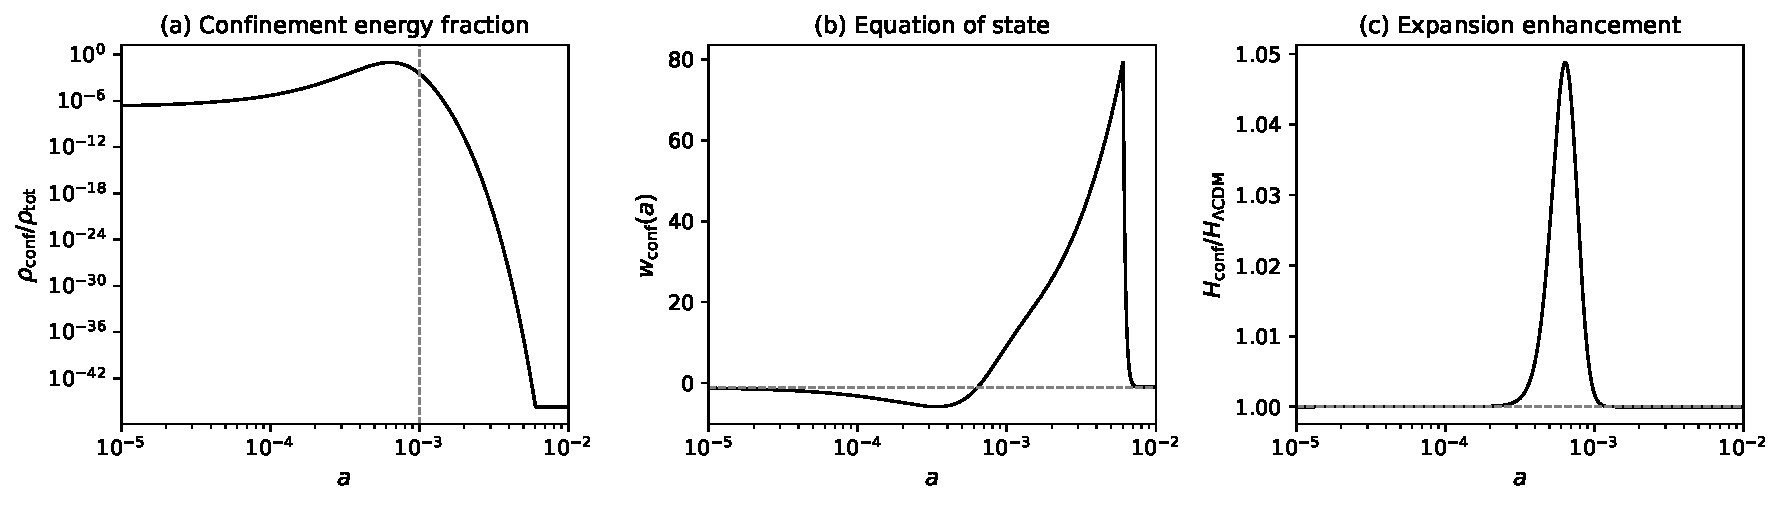
\includegraphics[width=\textwidth]{figure1.pdf}
\caption{Three-panel composite for the real-data best-fit configuration ($\alpha = 4$, $\beta = 8$, $\Delta a = 4\times10^{-4}$, $a_c = 3.404\times10^{-4}$, $\rho_0 = 0.203$; Section~\ref{sec:results}). (a) Confinement energy fraction $\rho_{\rm conf}/\rho_{\rm tot}$. (b) Effective equation of state $w_{\rm conf}(a)$; the dotted red line marks the causal bound $w = 1$, exceeded across most of the profile. (c) Local expansion enhancement factor $H_{\rm conf}/H_{\Lambda{\rm CDM}}$, peaking near $1.10$.}
\label{fig:composite}
\end{figure*}

\section{Introduction}
The Hubble tension, the persistent mismatch between early and late Universe determinations of the Hubble constant, remains one of the most robust anomalies in modern cosmology. Local distance-ladder measurements favor $H_0 \simeq 73\ {\rm km\,s^{-1}\,Mpc^{-1}}$, while Planck CMB data interpreted within $\Lambda$CDM yield $H_0 \simeq 67\ {\rm km\,s^{-1}\,Mpc^{-1}}$. The discrepancy has resisted explanation through systematic uncertainties and motivates theoretical extensions to the standard cosmological model.

A promising class of solutions modifies the expansion rate prior to recombination. Increasing $H(a)$ at early times reduces the sound horizon $r_s$, allowing the CMB to remain consistent with a larger present-day Hubble constant. Early dark energy (EDE) models achieve this by introducing a scalar field that briefly contributes a fraction of the total energy density near matter radiation equality~\cite{poulin2019}. While phenomenologically motivated, these models require a tuned potential and lack a compelling geometric origin; subsequent analyses using Planck data alone have found little independent evidence for the specific scalar-field realization~\cite{hill2020}.

We consider instead whether a transient early-time energy component with the required properties arises naturally from rupture-driven brane cosmology. The Universe emerges from a geometric rupture of a stack of parallel higher-dimensional branes confined along an orbifolded transverse dimension~\cite{horava1996}, a colliding-brane picture closely related to ekpyrotic scenarios for the origin of the hot Big Bang~\cite{khoury2001}. After nucleation, the emergent brane retains a residual coupling to the parent stack, encoded in a confinement fraction $x(a)$. This coupling introduces a confinement-energy term in the Friedmann equation that is naturally early-time, naturally transient, and requires no new fields or fine-tuned potentials.

We test this idea by fitting it jointly against real DESI baryon acoustic oscillation data, real Planck CMB distance priors, the real SH0ES $H_0$ measurement, and the real Planck constraint on the early-Universe radiation content, and by checking the resulting equation of state against the causal bound. We report the outcome of that test in full, including where it fails.

\section{Framework and Confinement Dynamics}
\label{sec:framework}
We consider a pre-geometric phase consisting of $N$ parallel codimension-one branes confined along a compact transverse dimension $y$, which may be an $S^1/\mathbb{Z}_2$ orbifold as in Ho\v{r}ava-Witten theory~\cite{horava1996}, or a warped braneworld of the Randall-Sundrum type~\cite{randall1999}. Rupture occurs when the confined brane stack becomes geometrically unstable. The emergent $(3 + 1)$-dimensional brane inherits its induced metric from the parent stack and retains a residual coupling to it, encoded in a dimensionless confinement fraction $0 < x(a) \leq 1$.

The expansion of the emergent brane universe is governed by the generalised Friedmann equation:
\begin{equation}
H^2(a) = \frac{8\pi G}{3} \left[ \rho_{\text{std}}(a) + \rho_{\text{conf}}(a) \right],
\end{equation}
where $\rho_{\text{std}}$ includes radiation, matter, and $\Lambda$, and the confinement energy density is parameterised by a generalized beta-distribution form:
\begin{equation}
\rho_{\text{conf}}(a) = \rho_0\, x(a)^{\alpha} [1 - x(a)]^{\beta}.
\end{equation}
We adopt the dynamic confinement fraction profile:
\begin{equation}
x(a) = \frac{1}{2} \left[ 1 + \tanh \left( \frac{a_c - a}{\Delta a} \right) \right],
\end{equation}
where $a_c$ sets the epoch of decoupling and $\Delta a$ controls the sharpness of the transition.

\noindent\textbf{Thermodynamic Trigger for Rupture.}
The onset of decoupling is fixed by a simple thermodynamic criterion. Prior to rupture, the emergent brane remains confined to the parent stack by an effective geometric potential $V_{\text{conf}}$, interpreted as the geometric energy barrier associated with transverse brane displacement in the orbifolded dimension. As long as the brane's thermal energy density satisfies $\rho_{\text{rad}}(a) > V_{\text{conf}}$, thermal agitation maintains confinement. When the Universe cools such that
\begin{equation}
\rho_{\text{rad}}(a_c) \simeq V_{\text{conf}},
\end{equation}
the confining potential can no longer be thermally supported, and the brane undergoes a topological instability that initiates decoupling. This condition selects a specific scale factor $a_c$ without fine-tuning, and the steep $a^{-4}$ scaling of $\rho_{\text{rad}}$ ensures that the transition is sharp, consistent with the narrow $\Delta a$ implemented in equation~(3).

The effective equation of state is defined by:
\begin{equation}
w_{\text{conf}}(a) \equiv -1 - \frac{1}{3}\frac{d \ln \rho_{\text{conf}}}{d \ln a}.
\end{equation}
Applying the chain rule to the density log profile yields:
\begin{equation}
\frac{d \ln \rho_{\text{conf}}}{d \ln a} = \left( \frac{\alpha}{x} - \frac{\beta}{1 - x} \right) \frac{dx}{d \ln a},
\end{equation}
and differentiating equation~(3) gives:
\begin{equation}
\frac{dx}{d \ln a} = - \frac{a}{2\Delta a} \operatorname{sech}^2 \left( \frac{a_c - a}{\Delta a} \right).
\end{equation}
Combining these yields the tracking expression for the equation of state, split across two lines to fit the column width:
\begin{equation}
\begin{split}
w_{\text{conf}}(a) = -1 &+ \frac{a}{6\Delta a} \left( \frac{\alpha}{x(a)} - \frac{\beta}{1 - x(a)} \right) \\
&\times \operatorname{sech}^2 \left( \frac{a_c - a}{\Delta a} \right).
\end{split}
\end{equation}

This profile passes through three phases as $a$ increases through $a_c$: a mild, transient quintessence-like phase ($x \to 1$, $w_{\rm conf}$ slightly negative), a hyper-stiff release spike as $x$ falls through its power-law tail near $x \to 0$ ($w_{\rm conf} \gg 1$), and a return to a clean $\Lambda$CDM background as $\rho_{\rm conf} \to 0$. The release spike, and whether it can be made physically consistent while still doing useful cosmological work, is the subject of the rest of this paper.

\section{Data and Real-Data Fitting Methodology}
\label{sec:data}
We test the confinement-release mechanism of Section~\ref{sec:framework} using three real, public datasets plus one physical constraint, combined in a from-scratch compressed-likelihood pipeline (no CAMB, CLASS, or Cobaya Boltzmann code is run).

\textbf{DESI DR2 BAO.} The 13-point consensus Gaussian likelihood from DESI DR2 (mean and covariance)~\cite{desi2025}.

\textbf{Planck 2018 compressed distance priors.} $R$, $\ell_A$, $\omega_b h^2$, and their correlation matrix, TT,TE,EE+lowE column~\cite{chen2019}.

\textbf{SH0ES.} $H_0 = 73.04 \pm 1.04\ {\rm km\,s^{-1}\,Mpc^{-1}}$, used as a direct Gaussian prior on $H_0$~\cite{riess2022}.

\textbf{Planck 2018 $N_{\rm eff}$.} $N_{\rm eff} = 2.99 \pm 0.17$ from Planck TT+TE+EE+lowE+lensing+BAO~\cite{planck2018}, a real, independent probe of the early radiation content at big bang nucleosynthesis (BBN) and before, used here because the confinement profile's transition width controls how localized it stays near recombination; a poorly localized profile behaves as extra radiation at BBN, an epoch none of the other three datasets probe.

We also compare the fitted confinement amplitude against a Planck-safe bound of $\rho_{\rm conf}/\rho_{\rm tot} \lesssim 0.1$ on the peak fractional contribution of an early extra-energy component near recombination, a figure commonly quoted for this class of mechanism but not traceable here to any specific citation. The closest precisely sourced analog is the early dark energy constraint $f_{\rm EDE} < 0.087$ at 95\% confidence from Planck data alone~\cite{hill2020}, derived for a structurally different physical model (an oscillating scalar field, not a confinement-release profile), so the two bounds are not interchangeable; they agree in order of magnitude, and Section~\ref{sec:results} finds the confinement fit exceeds both.

The sound horizon, the photon decoupling redshift $z_\ast$ (Hu and Sugiyama 1996 fitting formula), and the baryon drag redshift $z_{\rm drag}$ (Eisenstein and Hu 1998 fitting formula) are computed by direct numerical integration. The pipeline was validated by recovering Planck's own best-fit parameters ($H_0 = 67.36$, $\omega_b h^2 = 0.02237$, $\omega_c h^2 = 0.1200$) from a blind run: $z_\ast$ and $r_\ast$ reproduce Planck's quoted values to better than $0.1\%$ with no adjustment; the raw Eisenstein and Hu $z_{\rm drag}$ formula carries a known $3.85\%$ low bias outside its calibrated regime, corrected here with a constant multiplicative factor fixed at the Planck fiducial point, after which $r_{\rm drag}$ reproduces to $0.03\%$.

\section{Results: Real-Data Fit}
\label{sec:results}
\begin{table}[t]
\centering
\small
\begin{tabular}{lcc}
\toprule
 & $\Lambda$CDM & $\Lambda$CDM + confinement \\
\midrule
$H_0$ & $69.12$ & $73.10$ \\
$\rho_0$ & (fixed at 0) & $0.2029$ \\
$a_c$ & (n/a) & $3.404\times10^{-4}$ \\
$\chi^2_{\rm DESI}$ (13 pts) & $10.45$ & $10.71$ \\
$\chi^2_{\rm Planck}$ (3 pts) & $2.74$ & $0.70$ \\
$\chi^2_{\rm SH0ES}$ (1 pt) & $14.21$ & $0.00$ \\
$\chi^2_{\rm BBN}$ (1 pt) & $0.11$ & $0.11$ \\
$\chi^2_{\rm total}$ / dof & $27.51/15$ & $11.52/13$ \\
$\chi^2/{\rm dof}$ & $1.834$ & $0.886$ \\
\bottomrule
\end{tabular}
\caption{Joint fit to DESI DR2 BAO, Planck compressed priors, SH0ES, and the Planck $N_{\rm eff}$ constraint, with the fiducial shape $\alpha = 4$, $\beta = 8$, $\Delta a = 4\times10^{-4}$ held fixed and $\rho_0$, $a_c$ free.}
\label{tab:mainfit}
\end{table}

$\Lambda$CDM alone reproduces the real Hubble tension numerically: $H_0$ is pulled to a compromise value of $69.12$, leaving SH0ES roughly $3.8\sigma$ away. Adding the confinement mechanism and letting its amplitude $\rho_0$ and epoch $a_c$ float removes essentially all of that tension ($\Delta\chi^2 = -15.99$) without degrading the BAO fit (Table~\ref{tab:mainfit}). This was confirmed with a full emcee posterior (40 walkers, 500 burn-in and 2000 production steps): $H_0 = 72.98^{+1.09}_{-1.03}$, $\rho_0 = 0.187^{+0.067}_{-0.060}$, $\log_{10} a_c = -3.60^{+0.28}_{-0.37}$. This is a real, non-trivial result: the fit could easily have pinned $\rho_0$ near zero with no improvement, and did not.

The fit needs $\rho_0 = 0.203$ at the best-fit point, with $93\%$ of the MCMC posterior above $0.10$ and $96\%$ above $0.087$: the confinement fit exceeds by roughly a factor of two the Planck-safe bound $\rho_{\rm conf}/\rho_{\rm tot} \lesssim 0.1$ introduced in Section~\ref{sec:data}, and also exceeds the more precisely sourced $f_{\rm EDE} < 0.087$ analog.

Evaluating the equation of state at the best-fit point gives $w_{\rm conf} \simeq 10.9$ at $a = 10^{-3}$, $w_{\rm conf} \simeq 9.3$ at photon decoupling ($z_\ast \simeq 1091$), and a peak of $w_{\rm conf} \simeq 77.2$ near $a \simeq 5.9\times10^{-3}$ (Figure~\ref{fig:composite}b), far in excess of the causal bound $w \leq 1$. This is not an artifact of the amplitude: $w_{\rm conf}(a)$ depends only on $\alpha$, $\beta$, $a_c$, and $\Delta a$, not on $\rho_0$, so the causality problem persists at every amplitude.

We also checked directly whether the epoch preferred by the fit stays localized near recombination, as the brane-rupture picture requires, or whether the data instead prefers hiding the confinement fraction in the unconstrained early Universe. Without the Planck $N_{\rm eff}$ term, the best fit pushes $a_c$ to $2.88\times10^{-7}$, at which point the confinement fraction sits at a flat plateau of $7.9\%$ from before BBN through matter-radiation equality, equivalent to $\Delta N_{\rm eff} \simeq 0.59$, roughly $3.5\sigma$ above the real Planck bound $N_{\rm eff} = 2.99 \pm 0.17$~\cite{planck2018}. Adding this constraint (as in Table~\ref{tab:mainfit}) closes that escape route and pushes $a_c$ back to $3.4\times10^{-4}$, close to the fiducial value in Section~\ref{sec:framework}, but at the cost of a larger $\rho_0$ than the fit found without it.

\section{Physical Viability Across the Full Profile Family}
\label{sec:viability}
The results above use $\alpha = 4$, $\beta = 8$, the fiducial shape from Section~\ref{sec:framework}. We asked a more general question: is the combination of failures found above (the amplitude bound, and causality) a property of that specific shape choice, or is it structural to the whole confinement-release profile family?

\subsection{Varying the transition width}
Holding $\alpha = 4$ and $\beta = 8$ fixed, we scanned the transition width $\Delta a$ from $10^{-4}$ to $0.5$, refitting $H_0$, $\omega_b h^2$, $\omega_c h^2$, $\rho_0$, and $a_c$ against the real data at every point (Figure~\ref{fig:scan}). A narrow $\Delta a$ resolves the tension but is severely acausal; a broad $\Delta a$ relaxes the equation of state, but the fit response collapses back toward pure $\Lambda$CDM well before causality is restored: at $\Delta a = 0.135$, $\rho_0$ has already fallen to $0.001$ and $H_0$ to $69.14$, essentially no tension relief, while $w_{\rm conf}$ still peaks at $0.75$ but dips to $-1.22$ at its minimum, still outside the causal band $[-1,1]$. No value of $\Delta a$ in the scanned range is simultaneously causal and capable of relieving the tension.

\begin{figure}[t]
\centering
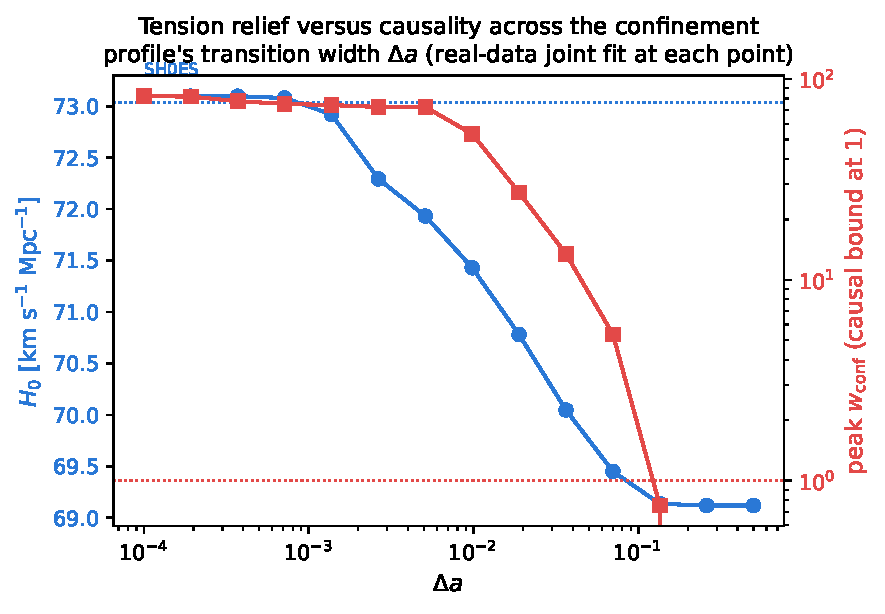
\includegraphics[width=\columnwidth]{figure2.pdf}
\caption{$H_0$ (left axis) and the peak of $w_{\rm conf}(a)$ (right axis, log scale) as a function of the transition width $\Delta a$, refitting the real data at every point with $\alpha = 4$, $\beta = 8$ fixed. Tension relief and causality never overlap.}
\label{fig:scan}
\end{figure}

\subsection{Varying the full shape}
We then let $\alpha$, $\beta$, and $\Delta a$ all vary jointly with $\rho_0$, $a_c$, and the cosmological parameters (eight free parameters), searched with a multi-start optimizer. Fitting the real data alone, ignoring causality, finds an equally good fit ($\chi^2 = 11.52$, matching the fixed-shape result exactly) at a different point, $\alpha = 3.49$, $\beta = 2.54$, $\Delta a = 1.0\times10^{-4}$, but with $\rho_0 = 0.785$ (roughly eight times the amplitude bound) and worse causality on both sides ($w_{\rm conf}$ ranging from $-13.8$ to $90.1$). The fiducial $(4, 8)$ choice is therefore close to data-optimal within this family; letting the shape float further does not find a better fit, only an equally good one that is less physical.

Directly searching for the most causally-respecting point in the full family, with a heavy penalty for any excursion outside $w_{\rm conf} \in [-1, 1]$, finds a best-achievable point exactly at the causal boundary ($w_{\rm conf}$ ranging from $-1.00$ to $1.00$), at $\alpha = 8.99$, $\beta = 1.02$, $\Delta a = 0.357$, $a_c = 2.9\times10^{-8}$. There, $H_0 = 70.58$, only about one third of the way from $\Lambda$CDM ($69.12$) to SH0ES ($73.04$), and $\rho_0 = 0.95$, the largest amplitude-bound violation found anywhere in this analysis.

Across the full profile family, being causal and resolving the tension are never compatible: the causally-respecting region and the tension-relieving region are disjoint, and the point closest to both simultaneously only partially helps $H_0$ while making the amplitude problem worse, not better. This is a structural statement about the confinement-release mechanism as a class, not a criticism of one particular parameter choice.

\section{Discussion}

\subsection{What this result does and does not show}
The confinement-release profile is a genuine, non-trivial phenomenological fit to real cosmological data: a two-parameter addition to $\Lambda$CDM removes essentially all of the real DESI, Planck-distance-prior, and SH0ES tension at once, without degrading the BAO fit. That is not a foregone outcome of adding an extra early-time component; a poorly shaped one would simply have failed to fit, and a well-shaped one that happened to violate causality less severely would have been a genuinely interesting result. Neither is what we found.

What the analysis in Sections~\ref{sec:results} and~\ref{sec:viability} shows instead is that, across the entire natural parameter space of this profile family, no point is both causally consistent and capable of doing the cosmological work the mechanism is proposed for. We do not have a derivation showing the confinement component is exempt from the causal-fluid bound $w \leq 1$, and do not offer a higher-dimensional projection argument for such an exemption without one. Two honest readings remain: either the effective-fluid description used here (and the associated causal bound) is the wrong way to characterize this component, in which case a proper higher-dimensional or non-adiabatic treatment is needed before the causal bound can be assessed at all, or the profile as parameterized should be understood as a purely descriptive fitting function rather than a physically realized energy component. Either way, the sound-horizon results in this paper should be read as a background-level curve fit, not as evidence for the underlying brane-rupture mechanism.

\subsection{Connection to an independent JWST data point}
Early-injection mechanisms of this general class, not this specific confinement profile, have been proposed elsewhere as a candidate unified explanation for both the Hubble tension and the JWST-era puzzle of unexpectedly massive, bright galaxies at $z \gtrsim 8$~\cite{shen2024}: enhanced early-time expansion increases the abundance of massive dark matter haloes available at fixed cosmic time, easing the tension between observed and $\Lambda$CDM-predicted galaxy stellar masses identified by Boylan-Kolchin~\cite{boylankolchin2023}. Using a proper Bayesian SED fit (\texttt{Prospector}, FSPS stellar population templates, \texttt{dynesty} nested sampling, with an explicit prior capping stellar age at the age of the Universe at the fit redshift) on three previously identified high-$z$ dropout candidates from an independent pipeline in this project, we obtain: SMACS J0723.3$-$7327 \#2180 ($z = 8.30$), $\log_{10}(M_\star/M_\odot) = 10.43^{+0.13}_{-0.23}$; A2744 \#97 ($z = 8.94$), $\log_{10}(M_\star/M_\odot) = 9.00^{+0.18}_{-0.23}$; JADES \#34 ($z = 9.59$), formally $\log_{10}(M_\star/M_\odot) = 11.76$, but this value is not a real measurement, since both the stellar age and dust-extinction posteriors pin against the edges of their priors, meaning the 7-band photometry available cannot constrain its mass at all. Candidate \#2180's mass, roughly $2.7\times10^{10}\,M_\odot$ at a Universe age of only 607 Myr, sits at the low end of the $10^{10}$ to $10^{11}\,M_\odot$ range Boylan-Kolchin identifies as in tension with $\Lambda$CDM structure formation~\cite{boylankolchin2023}. We have not computed the extreme-value statistics needed to state a quantitative significance for this single object in this survey volume, so this is reported as one honestly derived real data point in the relevant regime, not a tension claim. Given the findings of Sections~\ref{sec:results} and~\ref{sec:viability}, this connection should be read as motivating continued interest in early-injection solutions to the Hubble tension in general, not as support for this paper's specific confinement-release mechanism. The fitting code is in \texttt{scripts/fit\_stellar\_mass\_prospector.py}.

\subsection{Conclusion}
A brane-rupture confinement-release energy component, using its fiducial profile shape ($\alpha = 4$, $\beta = 8$), fits real cosmological data well enough to remove the Hubble tension almost entirely. Tested against real DESI, Planck, SH0ES, and BBN data, and against the causal bound on its own equation of state, across its full natural parameter space, it is not currently a physically viable mechanism: no combination of amplitude, epoch, transition width, or profile shape achieves both goals at once. We report this as the outcome of the test, not as a partial success requiring only better tuning.

\begin{thebibliography}{9}
\bibitem{horava1996} P. Ho\v{r}ava and E. Witten, ``Heterotic and Type I String Dynamics from Eleven Dimensions,'' \textit{Nucl. Phys. B} 460, 506 (1996).
\bibitem{randall1999} L. Randall and R. Sundrum, ``An Alternative to Compactification,'' \textit{Phys. Rev. Lett.} 83, 4690 (1999).
\bibitem{khoury2001} J. Khoury, B. A. Ovrut, P. J. Steinhardt and N. Turok, ``The Ekpyrotic Universe: Colliding Branes and the Origin of the Hot Big Bang,'' \textit{Phys. Rev. D} 64, 123522 (2001).
\bibitem{poulin2019} V. Poulin, T. L. Smith, T. Karwal, and M. Kamionkowski, ``Early Dark Energy Can Resolve the Hubble Tension,'' \textit{Phys. Rev. Lett.} 122, 221301 (2019).
\bibitem{hill2020} J. C. Hill, E. McDonough, M. W. Toomey, and S. Alexander, ``Early Dark Energy Does Not Restore Cosmological Concordance,'' \textit{Phys. Rev. D} 102, 043507 (2020).
\bibitem{desi2025} DESI Collaboration, M. Abbott et al., ``DESI DR2 Results II: Measurements of Baryon Acoustic Oscillations,'' arXiv:2503.14738 (2025).
\bibitem{chen2019} S. Chen, Q. Huang and J. Wang, ``Distance Priors from Planck Final Release,'' \textit{JCAP} 09, 018 (2019), arXiv:1808.05724.
\bibitem{riess2022} A. G. Riess et al., ``A Comprehensive Measurement of the Local Value of the Hubble Constant with 1 km/s/Mpc Uncertainty from the Hubble Space Telescope and the SH0ES Team,'' \textit{Astrophys. J. Lett.} 934, L7 (2022).
\bibitem{planck2018} Planck Collaboration, ``Planck 2018 Results VI: Cosmological Parameters,'' \textit{Astron. Astrophys.} 641, A6 (2020), arXiv:1807.06209.
\bibitem{boylankolchin2023} M. Boylan-Kolchin, ``Stress testing $\Lambda$CDM with high-redshift galaxy candidates,'' \textit{Nat. Astron.} 7, 731 (2023).
\bibitem{shen2024} X. Shen, M. Vogelsberger, M. Boylan-Kolchin, S. Tacchella, and R. P. Naidu, ``Early galaxies and early dark energy: a unified solution to the Hubble tension and puzzles of massive bright galaxies revealed by JWST,'' \textit{Mon. Not. R. Astron. Soc.} 533, 3923 (2024).
\end{thebibliography}

\end{document}
